% https://tex.stackexchange.com/questions/126144/how-to-draw-a-irregular-circleshape
\documentclass[border=3pt,tikz]{standalone}
\usepackage{tikz}
\usetikzlibrary{hobby}
\begin{document}

% https://en.wikibooks.org/wiki/LaTeX/PGF/TikZ#User-defined_paths
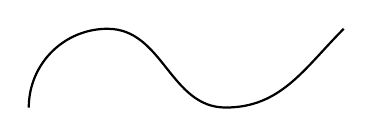
\begin{tikzpicture}
  \draw[thick] (0,0) to [out=90,in=180] (1,1)
               to [out=0,in=180] (2.5,0) to [out=0,in=-135] (4,1);
\end{tikzpicture}

% https://en.wikibooks.org/wiki/LaTeX/PGF/TikZ#Drawing_curved_paths
% https://en.wikipedia.org/wiki/B�zier_curve
\begin{tikzpicture}
  \draw[thick] (0,0) .. controls (1,1) .. (4,0) --
               (5,0) .. controls (6,0) and (6,1) .. (5,2);
\end{tikzpicture}

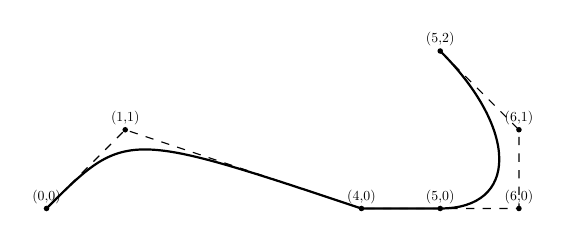
\begin{tikzpicture}
  \draw[thick] (0,0) .. controls (1,1) .. (4,0) --
               (5,0) .. controls (6,0) and (6,1) .. (5,2);
  
  \draw[dashed] (0,0) -- (1,1) -- (4,0) -- (5,0) -- (6,0) -- (6,1) -- (5,2);
  \foreach \p in {(0,0), (1,1), (4,0), (5,0), (6,0), (6,1), (5,2)}{
    \fill \p circle (1pt) node[above,scale=0.5] {\p};
  }
\end{tikzpicture}


\begin{tikzpicture}
  \draw plot[smooth, tension=.7] coordinates {(-3.5,0.5) (-3,2.5) (-1,3.5) (1.5,3) (4,3.5) (5,2.5) (5,0.5) (2.5,-2) (0,-0.5) (-3,-2) (-3.5,0.5)};
\end{tikzpicture}

\begin{tikzpicture}
  \draw  plot[smooth, tension=.8] coordinates {(-2.5,-0.5) (-3.5,0) (-2.5,0.5) (-3,1) (-2,1.5) (-2,3) (-1,2.5) (1,4.5) (2.5,3) (3,3.5) (3.5,3) (3,2) (4.5,2) (4.5,0) (3,1) (2.5,-0.5) (3.5,-1.5) (1.5,-1) (0.5,-2) (-2,-2.5) (-1.5,-1) (-2.5,-1.5) (-2.5,-0.5)};
\end{tikzpicture}



\begin{tikzpicture}[use Hobby shortcut,closed=true]
  \draw (-3.5,0.5) .. (-3,2.5) .. (-1,3.5).. (1.5,3).. (4,3.5).. (5,2.5).. (5,0.5) ..(2.5,-2).. (0,-0.5).. (-3,-2).. (-3.5,0.5);
\end{tikzpicture}

\begin{tikzpicture}[use Hobby shortcut,closed=true]
  \draw (-2.5,-0.5).. (-3.5,0).. (-2.5,0.5).. (-3,1).. (-2,1.5).. (-2,3).. (-1,2.5).. (1,4.5).. (2.5,3).. (3,3.5).. (3.5,3).. (3,2).. (4.5,2).. (4.5,0).. (3,1).. (2.5,-0.5).. (3.5,-1.5).. (1.5,-1).. (0.5,-2).. (-2,-2.5).. (-1.5,-1).. (-2.5,-1.5).. (-2.5,-0.5);
\end{tikzpicture}


\end{document}